\documentclass{article}
\usepackage{tabularx}
\usepackage{amsmath}
\usepackage{amssymb}
\usepackage{setspace}
\usepackage{color}
\usepackage{tikz}
\usepackage{graphicx}
\usepackage{tikz}
\usetikzlibrary{automata}
\usetikzlibrary{positioning}
\usetikzlibrary{arrows}
\tikzset{	node distance=2.5cm, 
	every state/.style={ 
		semithick,
		fill=gray!10},
	initial text={},     
	double distance=2pt, 
	every edge/.style={  
		draw,
		->, %>=stealth’,     
		auto,
		semithick}
}
\let\epsilon\varepsilon
\usepackage[margin=1in]{geometry}
\usepackage{xepersian}
\settextfont{Yas}
% Fixture for Xepersian 23 bug of setting persian math digit fonts
\ExplSyntaxOn \cs_set_eq:NN \etex_iffontchar:D \tex_iffontchar:D \ExplSyntaxOff
\setmathdigitfont{Yas}
\onehalfspacing
\newcommand*\circled[1]{
	\tikz[baseline=(char.base)]{
		\node[shape=circle,draw,inner sep=-1pt,color=red] (char) {\textcolor{black}{#1}\strut}
	}\kern-3pt
}
% Setup Enum
\renewcommand{\labelenumii}{\alph{enumii})}
\let\oldlabelenumi=\labelenumi
\let\oldlabelenumii=\labelenumii
% Enumi
\newcommand{\StartCircledEnumi}{\renewcommand{\labelenumi}{\circled{\oldlabelenumi}}}
\newcommand{\EndCircledEnumi}{\renewcommand{\labelenumi}{\oldlabelenumi}}
% Enumii
\newcommand{\StartCircledEnumii}{\renewcommand{\labelenumii}{\circled{\oldlabelenumii}}}
\newcommand{\EndCircledEnumii}{\renewcommand{\labelenumii}{\oldlabelenumii}}
\begin{document}
	\begin{center}
		\Huge
		مبانی نظریه محاسبه
	\end{center}
	\Large
	\begin{tabularx}{\linewidth}{>{\raggedleft\arraybackslash}X}
		کارگاه دوم
		\\
		مبحث: تعریف اتوماتای متناهی، پذیرش زبان اجتماع، اشتراک و تفاضل دو زبان
		\\
		
	\end{tabularx}
	\rule{\textwidth}{1pt}
	\large
	\begin{enumerate}
		\item 
		برای هر یک از زبان‌های
		$L \subseteq \{a, b\}^*$
		نشان دهید اعضای مجموعه 
		\lr{$\{a^n \; | \; n \geq 0\}$}
		نسبت به $L$ دو به دو قابل تشخیص
		\LTRfootnote{pairwise $L$-distinguishable}
		هستند و نتیجه بگیرید 
		\lr{DFA}
		برای آنها وجود ندارد.
		\begin{latin}
			\begin{enumerate}
				\item $L = \{a^nba^{2n} \; | \; n \geq 0\}$
				\item $L = \{a^ib^ja^k \; | \; k >  i + j \}$
				\item $L = \{a^ib^j \; | \; \text{$j = i$ or $j = 2i$}\}$
				\item $L = \{a^ib^j \; | \; \text{$j$ is multiple of $i$}\}$
				\item $L = \{x \in \{a,b\}^* \; | \; n_a(x) < 2n_b(x) \}$
				\item $L = \{x \in \{a,b\}^* \; | \; \text{no prefix of $x$ has more $b$'s than $a$'s} \}$
				\item $L = \{a^{n^3} \; | \;  n \geq 1\}$
				\item $L = \{ww \; | \;  w \in \{a,b\}^*\}$
			\end{enumerate}
		\end{latin}
		
		\item 
		اتوماتاهای متناهی $ M_1 $ در شکل \ref{M1} و $ M_2 $ در شکل \ref{M2} به ترتیب زبان های $L_1$  و $L_2$ را پذیرش
		\LTRfootnote{Accept}
		می‌کنند. برای هر یک از زبان های زیر اتوماتای پذیرنده آن را رسم کنید.
		
		
		
		\begin{enumerate}
			\item 
			$L_1 \cap L_2$
			\item 
			$L_1 \cup L_2$
			\item
			$L_1 - L_2$
		\end{enumerate}
		
		\begin{figure}[h]
			\begin{minipage}{0.5\textwidth}
				\centering
				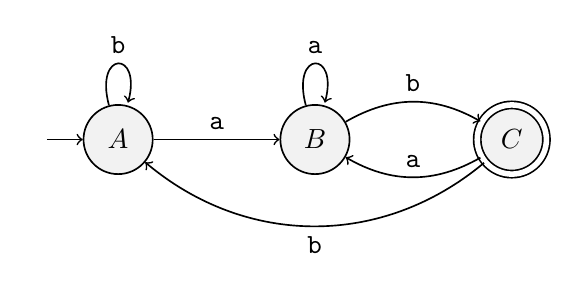
\begin{tikzpicture}
					\node[state, initial] (A) {$A$};
					\node[state, right of=A] (B) {$B$};
					\node[state, , accepting, right of=B] (C) {$C$};
					\draw (A) edge[loop above] node {\tt b} (A);
					\draw (B) edge[loop above] node {\tt a} (B);
					\draw (A) edge node {\tt a} (B);
					\draw (B) edge[bend left] node {\tt b} (C);
					\draw (C) edge[bend left] node [above] {\tt a} (B);
					\draw (C) edge[bend left = 40, below] node {\tt b} (A);
				\end{tikzpicture}
				\caption{$M_1$}
				\label{M1}
			\end{minipage}%
			\begin{minipage}{0.5\textwidth}
				\centering
				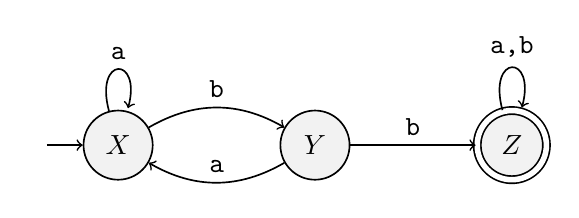
\begin{tikzpicture}
					\node[state, initial] (X) {$X$};
					\node[state, right of=X] (Y) {$Y$};
					\node[state, , accepting, right of=Y] (Z) {$Z$};
					\draw (X) edge[loop above] node {\tt a} (X);
					\draw (Z) edge[loop above] node {\tt a,b} (Z);
					\draw (Y) edge node {\tt b} (Z);
					\draw (X) edge[bend left] node {\tt b} (Y);
					\draw (Y) edge[bend left] node [above] {\tt a} (X);
				\end{tikzpicture}	
				\caption{$M_2$}
				\label{M2}	 		
			\end{minipage}
		\end{figure}
		
		
		\item 
		درستی یا نادرستی هر یک از گزاره‌های زیر را مشخص کنید. در صورت درستی، اثبات و در غیر این صورت مثال نقض ارائه کنید.
		\lr{($\Sigma = \{a, b\}$)}
		\begin{enumerate}
			\item 
			اگر  $ L_1 \subseteq L_2 $	، و $L_1 $  توسط  هیچ اتوماتی متناهی ای پذیرفته نشود، آنگاه $L_2 $  نیز توسط هیچ \lr{FA} ای پذیرفته نمی شود.
			\item 
			اگر  $ L_1 \subseteq L_2 $	، و $L_2 $  توسط  هیچ اتوماتی متناهی ای پذیرفته نشود، آنگاه $L_1 $  نیز توسط هیچ \lr{FA} ای پذیرفته نمی شود.
			\item 
			اگر $L_1 $ و $L_2 $ توسط هیچ \lr{FA} ای پذیرفته نشوند، آنگاه $ L_1 \cup L_2 $ نیز توسط هیچ \lr{FA} ای پذیرفته نمی شود.
			\item 
			اگر $L_1 $ و $L_2 $ توسط هیچ \lr{FA} ای پذیرفته نشوند، آنگاه $ L_1 \cap L_2 $ نیز توسط هیچ \lr{FA} ای پذیرفته نمی شود.
			\item 
			اگر $L $ توسط هیچ \lr{FA} ای پذیرفته نشود، آنگاه $ L ^ \prime $ نیز توسط هیچ \lr{FA} ای پذیرفته نمی شود.
			
			
			
		\end{enumerate}
		
	\end{enumerate}
	
	
\end{document}